\section{Lower Bounds and Trade-offs Between Robustness and Acceleration}

In the first part of this lecture, we study whether the convergence rates
derived in previous lectures are tight. For several classes of optimzation
problems (smooth, strongly convex, etc), we prove the
answer is indeed yes. The highlight of this analysis is to show the $O(1/t^2)$
rate achieved by Nesterov's accelerated gradient method is optimal (in a weak
technical sense) for smooth, convex functions. 

In the second part of this lecture, we go beyond studying convergence rates and
look towards other ways of comparing algorithms. We show the improved rates of
accelerated gradient methods come at a cost in robustness to noise. In
particular, if we restrict ourselves to only using approximate gradients, the
standard gradient method suffers basically no slowdown, whereas the accelerated
gradient method accumulates errors linearly in the number of iterations.

\subsection{Lower Bounds}
Before launching into a discussion of lower bounds, it's helpful to first recap
the upper bounds obtained thus far. For a convex function $f$,
Table~\eqref{table:upper-bounds} summarizes the assumptions and rates proved in
the first several lectures. 
~
\begin{table}[]
\centering
\caption{Upper Bounds from Lectures 2-8}
\label{table:upper-bounds}
\begin{tabular}{|l|l|l|}
\hline
$f$                        & Algorithm                    & Rate                                            \\ \hline
Convex, Lipschitz          & Gradient Descent             & $RL / \sqrt{t}$                               \\ \hline
Strongly Convex, Lipschitz & Gradient Descent             & $L^2 / (\alpha t)$                \\ \hline
Convex, Smooth             & Accelerated Gradient Descent & $\beta R^2 / t^2$ \\ \hline
\end{tabular}
\end{table}  

Each of the rates in Table~\eqref{table:upper-bounds} is obtained using some variant of the
gradient method. These algorithms can be thought of as a procedure that
maps a history of points and subgradients $(x_1, g_1, \dots, x_t, g_t)$ to a 
new point $x_{t+1}$. To prove lower bounds, we restrict the class of algorithms 
to similar procedures. Formally, define a black-box procedure as follows.

\begin{definition}[Black-Box Procedure]
A \textit{black-box procedure} generates a sequence of points $\set{x_t}$
such that
\begin{align*}
    x_{t+1} \in x_0 + \Span\set{g_1, \dots, g_t},
\end{align*}
and $g_s \in \partial f (x_s)$.
\end{definition}
Throughout, we will further assume $x_0 = 0$. As expected, gradient descent is a
black-box procedure. Indeed, unrolling the iterates, $x_{t+1}$ is given by
\begin{align*}
    x_{t+1} 
    &= x_t - \eta \grad f(x_t) \\
    &= x_{t-1} - \eta \grad f(x_{t-2}) - \eta \grad f(x_{t-1}) \\
    &= x_0 - \sum_{i=0}^t \eta \grad f (x_i).
\end{align*}

We now turn to proving lower bounds on the convergence rate for any 
black-box procedure.
Our first theorem concerns the constrained, non-smooth case.
The theorem is originally from \cite{nesterov83}, but the presentation will
follow \cite{nesterov04}.
~
\begin{theorem}[Constrainted, Non-Smooth $f$]\label{theorem:lb-non-smooth}
Let $t \leq n$, $L, R  > 0$. There exists a convex $L$-Lipschitz function $f$
such that any black-box procedure satisfies
\begin{align}
    \min_{1 \leq s \leq t} f(x_s) - \min_{x \in B_2(R)} f(x)
    \geq \frac{RL}{2(1+\sqrt{t})}.
\end{align}
Furthermore, there is an $\alpha$-strongly convex, $L$-Lipschitz function $f$
such that
\begin{align}
    \min_{1 \leq s \leq t} f(x_s) - \min_{x \in B_2(\frac{L}{2\alpha})} f(x)
    \geq \frac{L^2}{8\alpha t}.
\end{align}
\end{theorem}
The proof strategy is to exhibit a convex function $f$ so that, for any black-box procedure,
$\Span\set{g_1, g_2, \dots, g_i} \subset \Span\set{e_1, \dots, e_i}$, where
$e_i$ is the $i$-th standard basis vector. After $t$ steps for $t < n$, at least
$n-t$ coordinates are exactly 0, and the theorem follows from lower bounding the
error for each coordinate that is identically zero. 

\begin{proof}
Consider the function
\begin{align*}
    f(x) = \gamma \max_{1 \leq i \leq t} x[i] + \frac{\alpha}{2} \|x\|^2,
\end{align*}
for some $\gamma, \alpha \in \R$. In the strongly convex case, $\gamma$ is
a free parameter, and in the Lipschitz case both $\alpha$ and $\gamma$ are
free parameters. By the subdifferential calculus,
\begin{align*}
    \partial f(x) 
        = \alpha x + \gamma \conv\set{e_i \colon i \in \argmax_{1 \leq j \leq t} x(j)}.
\end{align*}
The function $f$ is evidently $\alpha$-strongly convex. Furthermore, if $\|x\| \leq R$
and $g \in \partial f(x)$, then $\|g\| \leq \alpha R + \gamma$, so $f$ is
$(\alpha R + \gamma)$-Lipschitz on $B_2(R)$.

Suppose the gradient oracle returns $g_i = \alpha x + \gamma e_i$, where
$i$ is the first coordinate such that $x[i] = \max_{1 \leq j \leq t} x[j]$. 
An inductive argument then shows
\begin{align*}
    x_s \in \Span\set{e_1, \dots, e_{s-1}}
\end{align*}
Consequently, for $s \leq t$, $f(x_s) \geq 0$. However, consider $y\in \R^n$
such that
\begin{align*}
    y[i] = 
    \begin{cases}
        -\frac{\gamma}{\alpha t} &\text{if } 1 \leq i \leq t\\
        0 &\text{otherwise}.
    \end{cases}
\end{align*}
Since $0 \in \partial f(y)$, $y$ is an minimizer of $f$ with objective value
\begin{align*}
    f(y)
    = \frac{-\gamma^2}{\alpha t} + \frac{\alpha}{2}\frac{\gamma^2}{\alpha^2 t}
    = -\frac{\gamma^2}{2\alpha t},
\end{align*}
and hence $f(x_s) - f(y) \geq \frac{\gamma^2}{2 \alpha t}$.
We conclude the proof by appropriately choosing $\alpha$ and $\gamma$. 
In the convex, Lipschitz case, set 
\begin{align*}
    \alpha = \frac{L}{R} \frac{1}{1 + \sqrt{t}}
    \quad
    \text{and}
    \quad
    \gamma = L \frac{\sqrt{t}}{1 + \sqrt{t}}.
\end{align*}
Then, $f$ is $L$-Lipschitz, 
\begin{align*}
    \norm{y} 
    = \sqrt{t \Paren{\frac{-\gamma}{\alpha t}}^2}
    = \frac{\gamma}{\alpha \sqrt{t}}
    = R
\end{align*}
and hence
\begin{align*}
    f(x_s) - \min_{x \in B_2(R)} f(x)
    = f(x_s) - f(y)
    \geq \frac{\gamma^2}{2\alpha t}
    = \frac{RL}{2(1+\sqrt{t})}.
\end{align*}
In the strongly-convex case, set $\gamma = \frac{L}{2}$ and take
$R = \frac{L}{2\alpha}$. Then, $f$ is $L$-Lipschitz, 
\begin{align*}
    \norm{y} 
    = \frac{\gamma}{\alpha \sqrt{t}}
    = \frac{L}{2\alpha \sqrt{t}}
    = \frac{R}{\sqrt{t}}
    \leq R,
\end{align*}
and therefore
\begin{align*}
    f(x_s) - \min_{x \in B_2(L/2\alpha)} f(x)
    = f(x_s) - f(y)
    \geq \frac{LR}{4t} 
    = \frac{L^2}{8\alpha t}.
\end{align*}
\end{proof}

Next, we study the smooth, convex case and show the $O(1/t^2)$ rate achieved by
accelerated gradient descent is optimal.

\begin{theorem}[Smooth-$f$]\label{theorem:lb-smooth}
Let $t \leq \frac{n-1}{2}$, $\beta > 0$. There exists a $\beta$-smooth convex
quadratic $f$ such that any black-box method satisfies
\begin{align}
    \min_{1 \leq s \leq t} f(x_s) - f(x^\star)
    \geq \frac{3\beta \norm{x_0 - x^\star}_2^2}{32(t+1)^2}.
\end{align}
\end{theorem}
Similar to the previous theorem, the proof strategy is to exhibit 
a pathological convex function. In this case, we choose what Nesterov calls
``the worst-function in the world'' \cite{nesterov04}.

\begin{proof}
Without loss of generality, let $n = 2t+1$.
Let $L \in \R^{n \times n}$ be the tri-diagonal matrix
\begin{align*}
    L =
    \begin{bmatrix}
        2 & -1 & 0 & 0 & \cdots & 0 \\
        -1 & 2 & -1 & 0 & \cdots & 0 \\
        0 & -1 & 2 & -1  & \cdots & 0 \\
        \vdots & \vdots & \vdots & \vdots & \ddots & \vdots \\
        0 & 0 & 0 & 0 & \cdots -1 & 2  \\
    \end{bmatrix}.
\end{align*}
The matrix $L$ is almost the Laplacian of the cycle
graph (in fact, it's the Laplacian of the chain graph).\footnote{\url{https://en.wikipedia.org/wiki/Laplacian_matrix}}
Notice
\begin{align*}
    x^\trans L x = x[1]^2 + x[n]^2 + \sum_{i=1}^{n-1} (x[i] - x[i+1])^2,
\end{align*}
and, from this expression, it's a simple to check
$0 \preceq L \preceq 4I$.
Define the following $\beta$-smooth convex function
\begin{align*}
    f(x) = \frac{\beta}{8} x^\trans L x - \frac{\beta}{4}\langle x, e_1 \rangle.
\end{align*}
The optimal solution $x^\star$ satisfies $Lx^\star = e_1$, and solving this 
system of equations gives
\begin{align*}
    x^\star[i] = 1 - \frac{i}{n+1},
\end{align*}
which has objective value
\begin{align*}
    f(x^\star)
    &=  \frac{\beta}{8} {x^\star}^\trans L x^\star - \frac{\beta}{4}\langle
    x^\star, e_1 \rangle \\
    &= -\frac{\beta}{8} \langle x^\star, e_1 \rangle
    = -\frac{\beta}{8} \paren{1 - \frac{1}{n+1}}.
\end{align*}
Similar to the proof of~\eqref{theorem:lb-non-smooth}, we can argue
\begin{align*}
    x_s \in \Span\set{e_1, \dots, e_{s-1}},
\end{align*}
so if $x_0 = 0$, then $x_s[i] = 0$ for $i \geq s$ for any black-box procedure.
Let $x_s^\star = \argmin_{x \colon i\geq s, x[i] = 0} f(x)$. Notice $x_s^\star$
is the solution of a smaller $s \times s$ Laplacian system formed by the
first $s$ rows and columns of $L$, so
\begin{align*}
    x_s^\star[i] = 
    \begin{cases}
        1- \frac{i}{s + 1} &\text{if } i < s \\
        0 &\text{otherwise},
    \end{cases}
\end{align*}
which has objective value $f(x_s^\star) = -\frac{\beta}{8}\paren{1 - \frac{1}{s + 1}}$.
Therefore, for any $s \leq t$,
\begin{align*}
    f(x_s) - f(x^\star) 
    &\geq f(x_t^\star) - f(x^\star) \\
    &\geq \frac{\beta}{8} \Paren{\frac{1}{t+1} - \frac{1}{n+1}} \\
    &= \frac{\beta}{8} \Paren{\frac{1}{t+1} - \frac{1}{2(t+1)}} \\
    &= \frac{\beta}{8}\frac{1}{2(t+1)}.
\end{align*}
To conclude, we bound the initial distance to the optimum. Recalling $x_0 = 0$,
\begin{align*}
    \norm{x_0 - x^\star}^2 =
    \norm{x^\star}^2 
    &= \sum_{i=1}^n \paren{1 - \frac{i}{n+1}}^2  \\
    &= n - \frac{2}{n+1} \sum_{i=1}^n i + \frac{1}{(n+1)^2} \sum_{i=1}^{n} i^2 \\
    &\leq n - \frac{2}{n+1} \sum_{i=1}^n i + \frac{1}{(n+1)^2} \int_1^{n+1} x^2 \, dx \\
    &\leq n - \frac{2}{n+1}\frac{n(n+1)}{2} + \frac{1}{(n+1)^2} \frac{(n+1)^3}{3} \\
    &= \frac{(n+1)}{3} \\
    &= \frac{2(t+1)}{3}.
\end{align*}
Combining the previous two displays, for any $s \leq t$,
\begin{align*}
    f(x_s) - f(x^\star)
    \geq \frac{\beta}{8}\frac{1}{2(t+1)} 
    \geq \frac{3 \beta\norm{x_0 - x^\star}^2}{32(t+1)^2}.
\end{align*}
\end{proof}

\subsection{Robustness and Acceleration Trade-offs}
The first part of the course focused almost exclusively on
convergence rates for optimization algorithms. From this
perspective, a better algorithm is one with a faster rate of convergence.
A theory of optimization algorithms that stops with rates of
convergence is incomplete. There are often other important algorithm design
goals, e.g. robustness to noise or numerical errors, that are ignored by
focusing on converges rates, and when these goals are of primary importance, 
excessive focus on rates can lead practitioners to choose the wrong algorithm.
This section deals with one such case.

In the narrow, technical sense of the previous section, Nesterov's Accelerated Gradient 
Descent is an ``optimal'' algorithm, equipped with matching upper and lower bounds on 
it's rate of convergence. A slavish focus on convergence rates suggests one should then
always use Nesterov's method. Before coronating Nesterov's method, however, it
is instructive to consider how it performs in the presence of noise.

Figure~\eqref{fig:nag-noise} shows compares the performance of vanilla gradient
descent and Nesterov's accelerated gradient descent on the function $f$ used in
the proof of Theorem~\eqref{thm:lb-smooth}. In the noiseless case, the
accelerated method obtains the expected speed-up over gradient descent. However,
if we add a small amount of spherical noise to the gradients, the speed-up not
only disappears, but gradient descent begins to outperform the accelerated
method, which begins to diverge after a large number of iterations.

\begin{figure}
\begin{center}
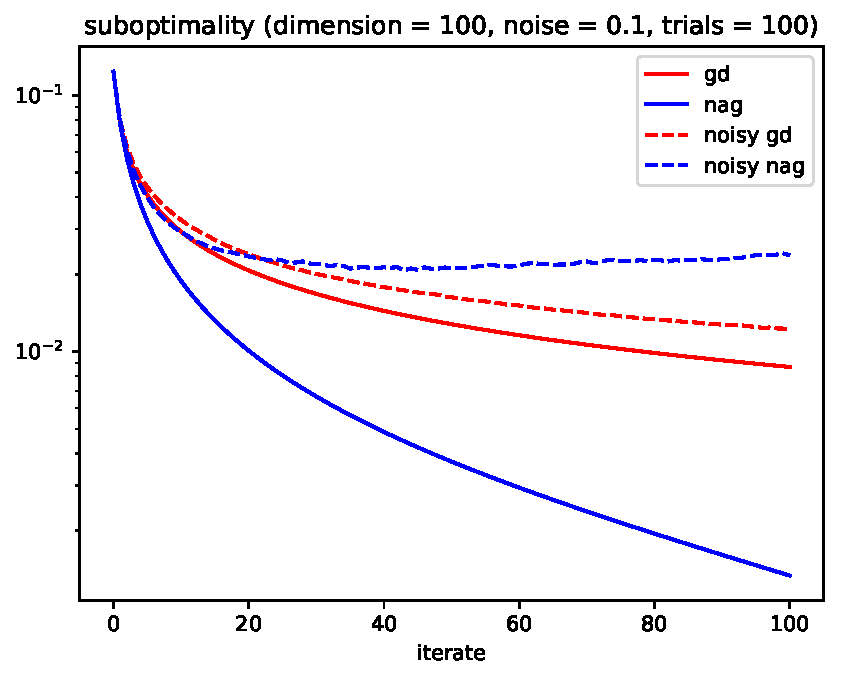
\includegraphics[width=3in]{figures/nag-noise.pdf}
\end{center}
\caption{The optimality gap for iterations of gradient descent and Nesterov accelerated gradient descent applied to the worst function in the world with dimension $n=100$. Notice with exact oracle gradients, acceleration helps significantly. However, when adding uniform spherical random noise with radius $\delta=0.1$ to the gradient, stochastic gradient descent remains robust while stochastic accelerated gradient accumulates error. The stochastic results are averaged over $100$ trials.}
\label{fig:nag-noise}
\end{figure}

The preceeding example is not wickedly pathological in any sense. Instead, it is
illustrative of a much broader phenomenon. Work by Devolder, Glineur and
Nesterov (DGN) \cite{devolder2014first} shows there is a
fundamental trade-off between acceleration and robustness, in a sense
made precise below. 

First, define the notion of an inexact gradient oracle. Recall for a
$\beta$-smooth convex function $f$ and any $x, y \in \domain$,
\begin{align}
    0 \leq f(x)  - \Paren{f(y) + \langle \grad f(y), x - y \rangle}
    \leq \frac{\beta}{2} \norm{x-y}^2. \label{eq:exact-oracle}
\end{align}
For any $y \in \domain$, an exact first-order oracle then returns a pair
$(f(y), g(y)) = (f(y), \grad f(y))$ that satisfies~\eqref{eq:exact-oracle}
exactly for every $x \in \domain$. 
An inexact oracle, returns a pair so that~\eqref{eq:exact-oracle} holds up to some
slack $\delta$.
~
\begin{definition}[Inexact-Oracle]
Let $\delta > 0$. For any $y\in \domain$, a $\delta$-inexact oracle returns a pair
$(f_\delta(y), g_\delta(y))$ such that
\begin{align*}
    0 \leq f(x)  - \Paren{f(y) + \langle \grad f(y), x - y \rangle}
    \leq \frac{\beta}{2} \norm{x-y}^2 + \delta
\end{align*}
for every $x \in \domain$.
\end{definition}
Consider running gradient descent with a $\delta$-inexact oracle.
DGN \cite{devolder2014first} show, after $t$ steps,
\begin{align*}
    f(x_t) - f(x^\star) \leq \frac{\beta R^2}{2t} + \delta.
\end{align*}
Comparing this rate with Table~\eqref{table:upper-bounds}, the plain gradient
method is not affected by the inexact oracle and doesn't accumulate errors. 
On the other hand, if the accelerated gradient
method is run with a $\delta$-inexact oracle, then after $t$ steps,
\begin{align*}
    f(x_t) - f(x^\star)  \leq \frac{4 \beta R^2}{(t+1)^2} +
    \frac{1}{3}(t+3)\delta.
\end{align*}
In other words, the accelerated gradient method accumulates errors linearly with
the number of steps! Moreover, this slack is not an artifact of the analysis.
Any black-box method must accumulate errors if it is accelerated in the exact
case, as the following theorem makes precise.
\begin{theorem}[\cite{devolder2014first} Theorem 6]
Consider a black-box method with convergence rate $O\Paren{\frac{\beta R^2}{t^p}}$
when using an exact oracle. With a $\delta$-inexact oracle, suppose the
algorithm achieves a rate
\begin{align}
    f(x_t) - f(x^\star) \leq O\Paren{\frac{\beta R^2}{t^p}} + O\Paren{t^q \delta},
\end{align}
then $q \geq p-1$.
\end{theorem}
In particular, for any accelerated method has $p > 1$, and consequently $q > 1$
so the method acculumates at least $O(t^{p-1} \delta)$ error with the number of
iterations. 
